\documentclass[]{article}
\usepackage[utf8]{inputenc}
\usepackage{amsmath}
\usepackage{amsfonts}
\usepackage{amssymb}
\usepackage{graphicx}

\title{Reporte 7}
\author{Antonio Cota Rodr\'iguez}
\date{}

\begin{document}
\maketitle

\section*{Introducci\'on}
La marea es el cambio periódico del nivel del mar producido principalmente por la fuerza de atracción gravitatoria que ejercen el Sol y la Luna sobre la Tierra. Aunque dicha atracción se ejerce sobre todo el planeta, tanto en su parte sólida como líquida y gaseosa, nos referiremos en este artículo a la atracción de la Luna y el Sol, juntos o por separado, sobre las aguas de los mares y océanos. Sin embargo, hay que indicar que las mareas de la litosfera son prácticamente insignificantes, con respecto a las que ocurren en el mar u océano (que pueden modificar su nivel en varios metros) y, sobre todo, en la atmósfera, donde puede variar en varios km de altura, aunque en este caso, es mucho mayor el aumento del espesor de la atmósfera producido por la fuerza centrífuga del movimiento de rotación en la zona ecuatorial (donde el espesor de la atmósfera es mucho mayor) que la modificación introducida por las mareas en dicha zona ecuatorial.

Otros fenómenos ocasionales, como los vientos, las lluvias, el desborde de ríos y los tsunamis provocan variaciones del nivel del mar, también ocasionales, pero no pueden ser calificados de mareas, pero que no están causados por la fuerza gravitatoria.

\section*{Teor\'ia de las mareas}

La teor\'ia din\'amica de las mareas describe y predice el comportamiento real de las olas en los oc\'eanos.
Mientras que Newton explicaba las mareas describiendo una fuerza generadora de las mareas y Bernoulli dio una descrpci\'on de la reacci\'on est\'atica del agua en la Tierra al potencial de marea, la teor\'ia din\'amica de las mareas, desarrollada por Pierre-Simon Laplace describe la reacci\'on real a las fuerzas de marea del oc\'eano. La teor\'ia de Laplace de los mareas de los oc\'eanos toma en cuenta la fricci\'on, resonancia y los periodos naturales de las cuencas oce\'anicas.

\section*{C\'odigo de Fortran}

A continuaci\'on se brindar\'a el c\'odigo para Fortran.

\begin{verbatim}

PROGRAM Mareas

IMPLICIT NONE
REAL, DIMENSION (7674):: altura
INTEGER :: i
!-------------------------------------
REAL :: Dif, Maxm1, Maxm2, Maxm3, Maxm4, Maxm5
REAL :: Tiempom1x, Tiempom2x, Tiempom3x, Tiempom4x, Tiempom5x
!-------------------------------------
REAL :: Dif2, Minm1, Minm2, Minm3, Minm4, Minm5
REAL :: Tiempom1n, Tiempom2n, Tiempom3n, Tiempom4n, Tiempom5n
!-------------------------------------
REAL :: Dif3, Maxd1, Maxd2, Maxd3, Maxd4, Maxd5
REAL :: Tiempod1x, Tiempod2x, Tiempod3x, Tiempod4x, Tiempod5x
!-------------------------------------
REAL :: Dif4, Mind1, Mind2, Mind3, Mind4, Mind5
REAL :: Tiempod1n, Tiempod2n, Tiempod3n, Tiempod4n, Tiempod5n
!-------------------------------------
REAL :: PeriodomM1, PeriodomM2, PeriodomM3, PeriodomM4, PeriodomM5
REAL :: PeriodomN1, PeriodomN2, PeriodomN3, PeriodomN4, Periodomn5
REAL :: PeriododM1, PeriododM2, PeriododM3, PeriododM4, PeriododM5
REAL :: PeriododN1, PeriododN2, PeriododN3, PeriododN4, PeriododN5
!--------------------------------------
REAL :: Periodo_mensual_max
REAL :: Periodo_mensual_min
REAL :: Periodo_diario_max
REAL :: Periodo_diario_min
!-------------------------------------




OPEN (1,file="Mareas.csv")

DO i=1,7674
READ (1,*) altura(i)
END DO
CLOSE (1)

Maxm1 = 0
DO i=1,1344
Dif=Maxm1 - altura(i)
IF (Dif < 0) THEN 
Maxm1 = altura (i)

Tiempom1x= i/48.0

END IF
END DO

Maxm2 = 0
DO i=1345,2690
Dif =  Maxm2 - altura(i)
IF (Dif < 0) THEN 
Maxm2 = altura(i)

Tiempom2x=i/48.0
END IF
END DO


Maxm3 = 0
DO i=2691,4035
Dif = Maxm3 - altura(i)
IF (Dif < 0) THEN 
Maxm3 = altura (i)

Tiempom3x=i/48.0
END IF
END DO 

Maxm4 = 0
DO i=4036,5380
Dif = Maxm4 - altura(i)
IF (Dif < 0) THEN 
Maxm4 = altura (i)

Tiempom4x=i/48.0
END IF
END DO

Maxm5 = 0
DO i=5381, 6725
Dif = Maxm5 - altura(i)
IF (Dif < 0) THEN 
Maxm5 = altura (i)

Tiempom5x=i/48.0
END IF
END DO

!---------------------------------------------

Minm1 = 0
DO i= 1, 1344
Dif2= Minm1 - altura(i)
IF (Dif2> 0) THEN 
Minm1 = altura (i)

Tiempom1n=i/48.0
END IF
END DO

Minm2 = 0
DO i= 1345, 2690
Dif2= Minm2 - altura(i)
IF (Dif2> 0) THEN 
Minm2 = altura (i)

Tiempom2n=i/48.0
END IF
END DO

Minm3 = 0
DO i= 2691, 4035
Dif2= Minm3 - altura(i)
IF (Dif2> 0) THEN 
Minm3 = altura (i)

Tiempom3n=i/48.0
END IF
END DO

Minm4 = 0
DO i= 4036, 5380
Dif2= Minm4 - altura(i)
IF (Dif2> 0) THEN 
Minm4 = altura (i)

Tiempom4n=i/48.0
END IF
END DO

Minm3 = 0
DO i= 5381, 6725
Dif2= Minm5 - altura(i)
IF (Dif2> 0) THEN 
Minm5 = altura (i)

Tiempom5n=i/48.0
END IF
END DO


!--------------------------------------------

Maxd1 = 0
DO i= 18, 65
Dif3= Maxd1- altura(i)
IF (Dif3< 0) THEN 
Maxd1 = altura (i)

Tiempod1x= i * 0.5

END IF
END DO

Maxd2 = 0
DO i= 66, 113
Dif2=  Maxd2 - altura(i)
IF (Dif3< 0) THEN 
Maxd2 = altura(i)

Tiempod2x=(i* 0.5)

END IF
END DO


Maxd3 = 0
DO i= 114, 161
Dif3= Maxd3 - altura(i)
IF (Dif3< 0) THEN 
Maxd3 = altura (i)

Tiempod3x=(i* 0.5)

END IF
END DO 

Maxd4 = 0
DO i= 162, 209
Dif3= Maxd4 - altura(i)
IF (Dif3< 0) THEN 
Maxd4 = altura (i)

Tiempod4x=(i* 0.5)

END IF
END DO 

Maxd5 = 0
DO i= 210, 257
Dif3= Maxd5 - altura(i)
IF (Dif3< 0) THEN 
Maxd5 = altura (i)

Tiempod5x=(i* 0.5)

END IF
END DO 

!--------------------------------------------

Mind1 = 0
DO i= 18, 65
Dif4= Mind1 - altura(i)
IF (Dif4> 0) THEN 
Mind1 = altura (i)

Tiempod1n=i * 0.5

END IF
END DO

Mind2 = 0
DO i= 66, 113
Dif4= Mind2 - altura(i)
IF (Dif2> 0) THEN 
Mind2 = altura (i)

Tiempod2n=( i * 0.5) 
END IF
END DO

Mind3 = 0
DO i= 114, 161
Dif4= Mind3 - altura(i)
IF (Dif4> 0) THEN 
Mind3 = altura (i)

Tiempod3n=(i* 0.5) 

END IF
END DO

Mind4 = 0
DO i= 162, 209
Dif4= Mind4 - altura(i)
IF (Dif4> 0) THEN 
Mind4 = altura (i)

Tiempod4n=(i* 0.5) 

END IF
END DO

Mind5 = 0
DO i= 210, 257
Dif4= Mind5 - altura(i)
IF (Dif4> 0) THEN 
Mind5 = altura (i)

Tiempod5n=(i* 0.5) 

END IF
END DO
!--------------------------------------------

PeriodomM1 = Tiempom1x 
PeriodomM2 = Tiempom2x - Tiempom1x
PeriodomM3 = Tiempom3x - Tiempom2x
PeriodomM4 = Tiempom4x - Tiempom3x
PeriodomM5 = Tiempom5x - Tiempom4x

PeriodomN1 = Tiempom1n 
PeriodomN2 = Tiempom2n - Tiempom1n
PeriodomN3 = Tiempom3n - Tiempom2n
PeriodomN4 = Tiempom4n - Tiempom3n
PeriodomN5 = Tiempom5n - Tiempom4n

PeriododM1 = Tiempod1x 
PeriododM2 = Tiempod2x - Tiempod1x
PeriododM3 = Tiempod3x - Tiempod2x
PeriododM4 = Tiempod4x - Tiempod3x
PeriododM5 = Tiempod5x - Tiempod4x

PeriododN1 = Tiempod1n 
PeriododN2 = Tiempod2n - Tiempod1n
PeriododN3 = Tiempod3n - Tiempod2n
PeriododN4 = Tiempod4n - Tiempod3n
PeriododN5 = Tiempod5n - Tiempod4n

!---------------------------------------------

Periodo_mensual_max = (PeriodomM1 + PeriodomM2 + PeriodomM3 + PeriodomM4 + PeriodomM5)/5.0

Periodo_mensual_min = (PeriodomN1 + PeriodomN2 + PeriodomN3 + PeriodomN4 + PeriodomN5)/5.0

Periodo_diario_max = (PeriododM1 +PeriododM2 +PeriododM3 + PeriododM4 + PeriododM5)/5.0

Periodo_diario_min = (PeriododN1 +PeriododN2 +PeriododN3 + PeriododN4 + PeriododN5)/5.0




Print *, 'Las mareas maximas mensuales fueron:'       
Print *, 'Primer mes:', Maxm1,'En el dia:', Tiempom1x
Print *, 'Segundo mes:',Maxm2,'En el dia:', Tiempom2x              
Print *, 'Tercer mes:',Maxm3,'En el dia:', Tiempom3x
Print *, 'Cuarto  mes:',Maxm4,'En el dia:', Tiempom4x             
Print *, 'Quinto mes:',Maxm5,'En el dia:', Tiempom5x

Print *, 'Las mareas minimas mensuales fueron:'
       
Print *, 'Primer mes:',Minm1, 'En el dia:', Tiempom1n
Print *, 'Segundo mes:',Minm2,'En el dia:', Tiempom2n           
Print *, 'Tercer mes:',Minm3,'En el dia:', Tiempom3n
Print *, 'Cuarto  mes:',Minm4,'En el dia:', Tiempom4n              
Print *, 'Quinto  mes:',Minm5,'En el dia:', Tiempom5n

Print *, 'El periodo mensual de la  marea  maxima  es:', Periodo_mensual_max, 'dias'

Print *, 'El periodo mensual de la marea minima es:', Periodo_mensual_min, 'dias'

Print *, 'Las mareas maximas diarias fueron:'       
Print *, 'Primer dia:', Maxd1
Print *, 'Segundo dia:',Maxd2           
Print *, 'Tercer dia:',Maxd3
Print *, 'Cuarto dia:',Maxd4           
Print *, 'Quinto dia:',Maxd5

Print *, 'Las mareas minimas diarias fueron:'     

Print *, 'Primer dia:',Mind1
Print *, 'Segundo dia:',Mind2             
Print *, 'Tercer dia:',Mind3
Print *, 'Cuarto dia:',Mind4              
Print *, 'Quinto dia:',Mind5


Print *, 'El periodo diario de la marea maxima es:', Periodo_diario_max, 'hrs'

Print *, 'El periodo diario de la marea  minima es:', Periodo_diario_min, 'hrs' 



end program Mareas

\end{verbatim}

\section*{An\'alisis de datos}
La siguiente imagen muestra los datos que se utilizar\'an para describir la variaci\'on del nivel del agua respecto al tiempo durante lo que dur\'o el experimento.

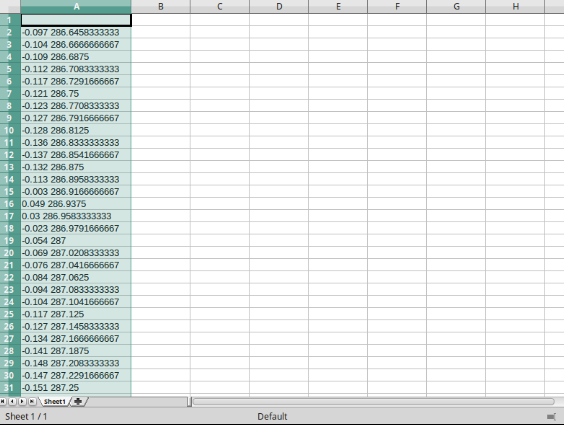
\includegraphics[scale=0.5]{Datos}\\

A continuaci\'on se muestra una imagen de los datos proporcionados por el programa en Fortran. 

\begin{center}
\includegraphics[scale=0.7]{Mareainf}\\
\end{center}

Al utilizar todos estos datos y el programa 'gnuplot' pasamos a graficar, con unos ejes adecuados queda de la siguiente manera:
\begin{center}
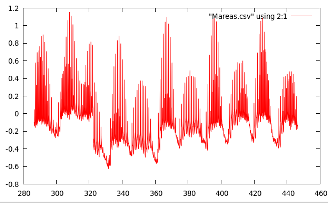
\includegraphics[scale=1]{GraficaMareas}
\end{center}


\end{document}